\section{Transmission Theory}\label{sec:theory}

\subsection{Similarity and Threshold Laws}\label{sec:similarity}

\begin{proposition}\label{prop:similarity}
Let Assumptions~\ref{ass:collinear} and~\ref{ass:wellposed} hold and let the neighbors remain taut. Define $\gamma = c/\sqrt{k m_L}$, $\gamma_L = c_L/\sqrt{k m_L}$ and $\gamma_A = c_A/\sqrt{k m_L}$. Every tension in \eqref{eq:model} equals $V\sqrt{k m_L}$ times a function of $t\sqrt{k/m_L}$ that depends only on $m_A/m_L$, $N$, $\gamma$, $\gamma_L$ and $\gamma_A$. Consequently $\rho=\Phi(m_A/m_L,N,\gamma,\gamma_L,\gamma_A)$ for a function $\Phi$ that does not depend on $V$, $k$ or $\Tn$ separately, and without dissipation $\rho$ depends on $m_A/m_L$ and $N$ alone.
\end{proposition}

\begin{proof}
Set $\ell=V\sqrt{m_L/k}$ and $s=t\sqrt{k/m_L}$, with $x=\ell\xi$, $y=\ell\eta$, and $y_j=\ell\eta_j$. Inertial, spring, and damping terms in \eqref{eq:model} share the force scale $k\ell=V\sqrt{k m_L}$; after division by it, the equations and switching surface depend only on $r=m_A/m_L$, $N$, $\gamma$, $\gamma_L$, and $\gamma_A$, with $\eta_j'(0)=1$. Uniqueness fixes the corresponding dimensionless response. Since both $f$ and $\delta T$ scale by $k\ell$, their peak ratio has the stated dependence, and $\Tn$ does not enter \eqref{eq:model}.
\end{proof}

Without solving \eqref{eq:model}, the proposition predicts that stiffness can change the transmission only through the three dissipation numbers, which fall as $k^{-1/2}$; an undamped law such as \eqref{eq:imp} cannot depend on stiffness at all (tested in Section~\ref{sec:stiffness}). The same scaling gives an exact criterion for slackening a neighbor, that is, for its tension to reach zero. Let $\bar T_{\mathrm p}$ denote the peak that the taut model \eqref{eq:model} assigns to a given closing speed; it equals the actual peak whenever the neighbors stay taut.

\begin{corollary}\label{cor:threshold}
Under Assumptions~\ref{ass:collinear} and~\ref{ass:wellposed}, a snap slackens the neighbors if and only if $\rho\,\bar T_{\mathrm p}\ge\Tn$.
\end{corollary}

\begin{proof}
The minimum taut-model tension is $\Tn-\rho\bar T_{\mathrm p}$. If positive, uniqueness keeps the actual solution taut. Otherwise, the actual and taut solutions coincide until the first zero of $\Tn+\delta T$, so the neighbor reaches zero tension.
\end{proof}

\noindent\textit{Control implication.}
Since $\Tn$ does not enter \eqref{eq:model}, the proof extends to unequal pretensions $T_{\mathrm{n},i}$: no neighbor slackens if and only if $\rho\,\bar T_{\mathrm p}<\min_i T_{\mathrm{n},i}$. The bound is joint, since once a weaker neighbor slackens the others unload further, so a pretension or allocation policy must enforce it for all neighbors at once, with $\bar T_{\mathrm p}\propto V$ predicted from the anticipated closing speed (Proposition~\ref{prop:similarity}) and a margin for model error.

\subsection{Closed Form Under the Contact Pulse}\label{sec:closedform}

To obtain $\rho$ in closed form, we replace the self-consistent contact by the isolated-pair pulse of \eqref{eq:imp} and set aside dissipation; Sections~\ref{sec:selfconsistent} and~\ref{sec:dissipation} restore both. The ratio of the peak half-sine response of a linear oscillator to its impulsive response is the pulse's shock spectrum \cite{harris2002shock}; we need it with an argument that identifies which extremum is the peak.

\begin{lemma}\label{lem:spectrum}
Let $0<\varepsilon\le 3$ and let $u$ solve $\ddot u+\varepsilon^2u=\sin t$ on $[0,\pi]$ and $\ddot u+\varepsilon^2u=0$ afterwards, with $u(0)=\dot u(0)=0$. Then $\sup_{t\ge0}|u(t)| = 2S(\varepsilon)/\varepsilon$, where
\begin{equation}\label{eq:spectrum}
  S(\varepsilon) =
  \begin{cases}
    \dfrac{\cos(\pi\varepsilon/2)}{1-\varepsilon^2}, & \varepsilon<1,\\[4pt]
    \pi/4, & \varepsilon = 1,\\[2pt]
    \dfrac{\sin\!\big(2\pi/(1+\varepsilon)\big)}{2(\varepsilon-1)}, & 1<\varepsilon\le 3.
  \end{cases}
\end{equation}
Moreover $S(\varepsilon)\to1$ as $\varepsilon\to0$, and $S$ decreases on $[1,3]$ from $\pi/4$ to $1/4$.
\end{lemma}

Since the same impulse, $\int_0^\pi\sin t\,dt=2$, applied at $t=0$ gives amplitude $2/\varepsilon$, $S$ is the peak relative to the impulsive one.

\begin{proof}
For $\varepsilon\neq1$,
\begin{equation*}
 u=\frac{\sin\varepsilon t-\varepsilon\sin t}{\varepsilon(1-\varepsilon^2)},\qquad
 \dot u=\frac{2\sin\frac{(1+\varepsilon)t}{2}\sin\frac{(1-\varepsilon)t}{2}}{1-\varepsilon^2}.
\end{equation*}
The energy $E=u^2+\dot u^2/\varepsilon^2$ satisfies $\dot E=2\dot u\sin t/\varepsilon^2$ on $[0,\pi]$, is constant afterwards, and bounds $|u|\le\sqrt E$. For $\varepsilon<1$, both sine factors are positive on $(0,\pi]$, so $\dot u>0$, $E$ is nondecreasing, and the supremum is $\sqrt{E(\pi)}$. For $1<\varepsilon\le3$, $\sin((\varepsilon-1)t/2)>0$ on $(0,\pi)$, while $\sin((1+\varepsilon)t/2)$ is positive before $t^*=2\pi/(1+\varepsilon)$ and, because $(1+\varepsilon)\pi/2\le2\pi$, nonpositive on $[t^*,\pi]$; hence $u$ increases to $t^*$, $E$ is nonincreasing afterwards, and $|u(t)|\le\sqrt{E(t^*)}=u(t^*)=\sin t^*/(\varepsilon(\varepsilon-1))$ for $t\ge t^*$, using $\varepsilon t^*=2\pi-t^*$. At $\varepsilon=1$, $u=(\sin t-t\cos t)/2$ with $\dot u=(t\sin t)/2\ge0$, so the supremum is $\sqrt{E(\pi)}=\pi/2$. Dividing by $2/\varepsilon$ gives \eqref{eq:spectrum}. On $(1,3]$, $w=\pi-t^*\in(0,\pi/2]$ increases with $\varepsilon$ and $S=(\pi-w)\sin w/(4w)$, whose $w$-derivative has the sign of $w(\pi-w)\cos w-\pi\sin w<0$, since $\pi\sin w\ge\pi w\cos w>(\pi-w)w\cos w$ for $\cos w>0$ and the first term vanishes at $w=\pi/2$.
\end{proof}

\begin{theorem}\label{thm:closedform}
Let Assumption~\ref{ass:collinear} hold with $c=c_L=c_A=0$, and replace the contact force in \eqref{eq:model} by $f(t)=\Tp\sin\omega_e t$ on $[0,\pi/\omega_e]$ and $f=0$ afterwards. Let $\omega_q=\omega_L$ if the neighbor vessels are held and $\omega_q=\omega_f\coloneqq\sqrt{k((N-1)/m_L+1/m_A)}$ if they are free. If $\varepsilon_q\coloneqq\omega_q/\omega_e\le3$, then
\begin{equation}\label{eq:closedform}
  \rho = \frac{2k}{m_L\,\omega_q\,\omega_e}\,S(\varepsilon_q).
\end{equation}
\end{theorem}

\begin{proof}
For $q=x-y$, \eqref{eq:model} gives $\ddot q+\omega_q^2q=f/m_L$ (with $q=x$ when held) and $\Delta T=kq$. Setting $s=\omega_e t$ and $q=\Tp u(s)/(m_L\omega_e^2)$ reduces the response to Lemma~\ref{lem:spectrum}, yielding \eqref{eq:closedform}.
\end{proof}

The prefactor in \eqref{eq:closedform} is the impulsive transmission of the same fleet, and \eqref{eq:imp} is the held case with $S=1$. With free far ends and $N\le10$, the theorem holds for every choice of masses:

\begin{corollary}\label{cor:unreachable}
With free far ends and the half-sine pulse of Theorem~\ref{thm:closedform},
\begin{equation}\label{eq:free}
\begin{aligned}
  \frac{2k}{m_L\omega_f\omega_e} &= \frac{2m_A}{\sqrt{(m_A+m_L)(m_L+(N-1)m_A)}},\\
  \varepsilon_f^2 &= 1+\frac{(N-2)\,m_A}{m_A+m_L}.
\end{aligned}
\end{equation}
Hence for $2\le N\le10$ and all masses $\varepsilon_f\ge1$, with $\varepsilon_f=1$ when $N=2$ and $1<\varepsilon_f<\sqrt{N-1}\le3$ when $N\ge3$, and that pulse removes at least $1-\pi/4\approx21\%$ of the corresponding impulsive transmission $2k/(m_L\omega_f\omega_e)$, with equality only for $N=2$; since $\omega_f>\omega_L$, the free-end law \eqref{eq:closedform} lies more than $1-\pi/4$ below \eqref{eq:imp}.
\end{corollary}

\begin{proof}
Substitution gives \eqref{eq:free}. Thus $\varepsilon_f=1$ for $N=2$ and $1<\varepsilon_f<\sqrt{N-1}\le3$ for $3\le N\le10$; Lemma~\ref{lem:spectrum} then gives $S(\varepsilon_f)\le S(1)=\pi/4$.
\end{proof}

\begin{figure}[t]
  \centering
  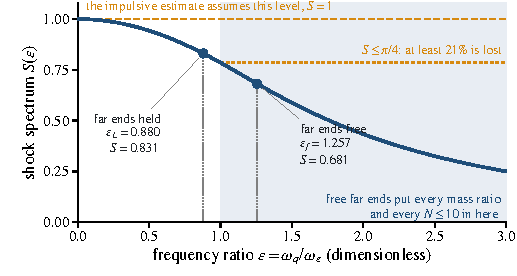
\includegraphics[width=\columnwidth]{fig_shock_spectrum}
  \caption{Half-sine shock spectrum $S(\varepsilon)$: the peak response to the pulse relative to the same impulse delivered instantly; \eqref{eq:imp} assumes $S=1$. Held far ends put the testbed at $\varepsilon_L=0.880$, $S=0.831$; free far ends force $\varepsilon_f\ge1$, so $S\le\pi/4$ for $N\le10$, and put the testbed at $\varepsilon_f=1.257$, $S=0.681$.}
  \label{fig:spectrum}
\end{figure}

The impulsive regime needs $\varepsilon_q\to0$, but with free far ends the neighbor mode is never slower than the pulse (Fig.~\ref{fig:spectrum}). The held case shows why \eqref{eq:imp} cannot be rescued by choosing the masses: $\varepsilon_L^2=(N-1)m_A/(m_A+m_L)$ is small, and the contact nearly impulsive, only when $m_A\ll m_L/(N-1)$, whereas held far ends require $\omega_f\approx\omega_L$, that is $m_A\gg m_L/(N-1)$. The two hypotheses demand opposite mass ratios, and the testbed, with $m_A/m_L=0.24$ against $1/(N-1)=0.25$, satisfies neither. Removing them one at a time, the finite pulse costs 17\% of \eqref{eq:imp}; the recoil of the far ends removes a further 43\% of what remains, and damping and drag 21\% of the rest, while the pulse shape assumed in Theorem~\ref{thm:closedform} changes the result by 1--2\%.

\subsection{Self-Consistent Contact Across Mass Ratios}\label{sec:selfconsistent}

We integrate \eqref{eq:model} with its unilateral force (adaptive RK4(5), relative tolerance $10^{-10}$, maximum step $\pi/(800\omega_e)$); with the prescribed pulse instead, this reproduces \eqref{eq:closedform} to six digits. For five cables the half-sine law is within $1.7$\% of the undamped self-consistent ratio for $m_A/m_L\le1$; the latter rises with vessel mass while far-end recoil dominates and falls once the lengthening contact does, with a secondary rise beyond $m_A/m_L\approx5$ (Fig.~\ref{fig:massratio}). We evaluate it on a 31-point logarithmic grid of $m_A/m_L$ over $[10^{-1.5},10^{1.5}]$ and refine the grid maximum by a bounded Brent search to $10^{-3}$. For $N=5$ this gives $\rho^\star=0.367$ at $m_A/m_L=1.41$, a numerical maximum, not a proof; by Corollary~\ref{cor:threshold}, no snap with $\bar T_{\mathrm p}<\Tn/\rho^\star\approx2.73\Tn$ slackens a neighbor in the undamped collinear model. For $N=3$--$8$ (Table~\ref{tab:worst}), every maximum lies more than a decade inside the interval and $(N-1)\rho^\star$ decreases monotonically from $1.54$ to $1.42$; whether this reflects a bound $\rho^\star\lesssim C/(N-1)$ is open, and for $N=2$ the search gives $\rho^\star=1.41$ at $m_A/m_L=4.0$.
\begin{figure}[t]
  \centering
  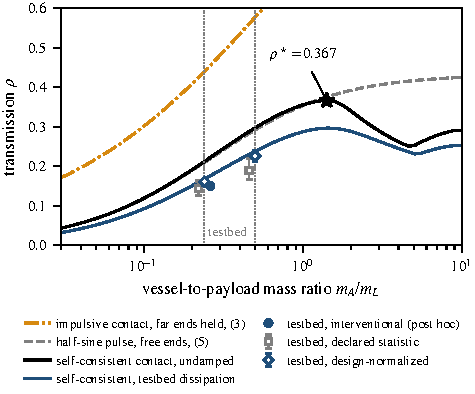
\includegraphics[width=\columnwidth]{fig_massratio}
  \caption{Five-cable transmission versus mass ratio. The undamped self-consistent contact has a numerical interior maximum $\rho^\star=0.367$ (star); the half-sine law tracks it for $m_A/m_L\le1$. Testbed markers, for the nominal cell of Section~\ref{sec:test} and its paired cell at $m_A=1250$\,kg: the recorded-geometry statistic (squares) and the design-normalized statistic (diamonds), both with seed intervals, the latter post hoc at $0.24$ and the declared primary of the second-mass test at $0.50$; and, at $0.24$, the post hoc interventional swing (circle).}
  \label{fig:massratio}
\end{figure}

\begin{table}[t]
  \caption{Largest Undamped Self-Consistent Transmission in the Mass-Ratio Search}
  \label{tab:worst}
  \centering
  \begin{tabular}{ccccc}
    \toprule
    $N$ & $m_A/m_L$ at max & $\rho^\star$ & $1/\rho^\star$ & $(N-1)\rho^\star$ \\
    \midrule
    3 & 2.67 & 0.770 & 1.30 & 1.54 \\
    4 & 1.94 & 0.501 & 2.00 & 1.50 \\
    5 & 1.41 & 0.367 & 2.73 & 1.47 \\
    6 & 1.11 & 0.289 & 3.46 & 1.45 \\
    7 & 0.92 & 0.239 & 4.19 & 1.43 \\
    8 & 0.78 & 0.203 & 4.92 & 1.42 \\
    \bottomrule
  \end{tabular}
\end{table}

\subsection{Dissipation and Stiffness}\label{sec:dissipation}

With the testbed's cable damping and drag (Table~\ref{tab:plant}), the self-consistent ratio is $0.167$ and the half-sine ratio $0.165$; the latter coincides to six digits with the planar forecast committed for the test of Section~\ref{sec:test}. By Proposition~\ref{prop:similarity} the stiffness enters only through the dissipation numbers, which yields two predictions. First, quartering and quadrupling $k$ moves $\rho$ from $0.139$ to $0.184$ under the half-sine pulse and from $0.140$ to $0.186$ self-consistently, increases of $0.045$ and $0.046$, whereas every undamped law, \eqref{eq:imp} and \eqref{eq:closedform} included, predicts none. Second, the swing's extremum, which Lemma~\ref{lem:spectrum} places at $2\pi/((1+\varepsilon_f)\omega_e)=149$\,ms without dissipation and which then scales as $k^{-1/2}$, arrives earlier with dissipation and scales more weakly: at $k/4$, $k$ and $4k$ the model places it at $205$, $125$ and $69$\,ms self-consistently and at $250$, $135$ and $71$\,ms under the half-sine pulse. Only the half-sine values of the first prediction were committed before the campaign, as the planar forecast; the self-consistent and timing values were computed after the measurements of Section~\mbox{\ref{sec:stiffness}}.
